\section{Nondegeneration of the electrical networks}
\label{sec:nondegeneration}

We first prove that a fixed conformal annulus admits cutoffs of bounded
electrical energy on both sewn graphs.  The bound will depend on the
annulus aspect and the coordinate patch, but not on its radius or the
discrete resolution.  This is the coercivity input for the variational
argument in the next section.  Throughout this section we work with
the bilateral sewing, at rates $m\to\infty$, and use the coupled
extractions and projections $\pi_m$ of
Proposition~\ref{inp:array-interface}.

The proof combines two uses of extremal length.  A lower bound supplies
densities that charge every crossing of an annulus.  If lower bounds
failed, a suitable quantile would instead supply probability measures
on crossing paths with very small squared traffic.  Annular densities
make their projected limits rectifiable.  Locality then forces a
transverse crossing witness on the other graph, contradicting the
small traffic.  The annular-density, rectifiable-flow, and local-germ
strategy is developed for flag extremal length in
\cite[Section ``The canonical conformal structure'']{ConformalMaps}.
We adapt it to edge energies on paired primal and dual graphs.

\subsection{Extremal length and local germs}

Let $\mathcal P$ be a nonempty family of paths in a finite graph, with
no path of length zero.  Edge occurrences are counted with
multiplicity.  Its edge extremal length is
\begin{equation}\label{nd:el-definition}
 \EL(\mathcal P)
 =\sup_{a:E\to[0,\infty)}
   \frac{\bigl(\inf_{P\in\mathcal P}\sum_{e\in P}a(e)\bigr)^2}
        {\sum_{e\in E}a(e)^2},
\end{equation}
where the zero density is omitted.  For a probability measure $\nu$
on paths, write
$j_\nu(e)=\int \#\{\text{occurrences of }e\text{ in }P\}\,\nu(\dd P)$
for its unsigned edge traffic.

\begin{lemma}[Densities and traffic]\label{nd:el-traffic}
For a finite family of simple paths,
\begin{equation}\label{nd:traffic-identity}
 \EL(\mathcal P)=\min_{\nu}\sum_e j_\nu(e)^2.
\end{equation}
If $\mathcal P$ consists of all paths between two disjoint wired sets
in a finite subgraph, then $\EL(\mathcal P)$ is the reciprocal of
the minimum energy $\en(u)$ subject to the values zero and one on
the two sets.  In particular, $\EL(\mathcal P)\ge b>0$ supplies a
density charging each path by one with squared norm at most $1/b$.
\end{lemma}

\begin{proof}
The traffic vectors form the convex hull of the path-incidence
vectors.  Let $j$ be its point nearest to the origin.  The supporting
inequality $\langle j,j_P\rangle\ge\|j\|_2^2$ for every path $P$
shows that the density $j$ gives a value at least $\|j\|_2^2$ in
\eqref{nd:el-definition}.  Conversely, averaging path length under
any $\nu$ and applying Cauchy--Schwarz gives
$\EL(\mathcal P)\le\|j_\nu\|_2^2$.  This proves
\eqref{nd:traffic-identity}.  In the wired-set case loops may be
removed from paths.  Absolute potential increments give a charging
density, while the distance from the first set in any charging
density, clipped at one, gives an admissible potential whose energy
is at most the squared density norm.  These two constructions prove
the reciprocal identity.
\end{proof}

We will also use a consequence of the local conditional kernels from
Section~\ref{sec:inputs}.  A \emph{point-germ readout} is a jointly
measurable random function $Y(z)$ whose value at $z$ can be read from
the fields and extracted arrays in every neighborhood of $z$.  The
readout may use countably many tests with strictly positive domain
margins.  In particular, an assertion that specified tests succeed
at every sufficiently small scale is a point-germ readout.

\begin{lemma}[Determinism of point germs]\label{nd:germs}
In an ordinary field chart, every bounded real point-germ readout
of the extracted local arrays is, almost surely, equal at
Lebesgue-almost every point to a deterministic measurable function
of the point.  The same conclusion holds for readouts with values
in a separable metric space, using a countable family of bounded
coordinates that separates its points.
\end{lemma}

\begin{proof}
Let $\mathcal H$ denote the pair of fields.  By
Proposition~\ref{inp:local-kernels},
$\E[Y(z)\mid\mathcal H]$ is measurable with respect to the field
restrictions to every neighborhood of $z$.  This field germ is
trivial.  Indeed, for a zero-boundary Gaussian free field, the
intersection of the Gaussian subspaces generated by restrictions
to shrinking disks is orthogonal to the Gaussian variables
associated with Dirichlet functions vanishing near $z$.  Such
functions are dense in the Dirichlet space: logarithmic cutoffs
express the zero capacity of a point.  The intersection is thus
zero, and the Gaussian chaos decomposition gives triviality of
the corresponding sigma-field.  Apply this to both independent
fields.  Local equivalence in Lemma~\ref{inp:gaussian}
transfers the conclusion to the ordinary chart, including the
imaginary field modulo its period.  Consequently
$\E[Y(z)\mid\mathcal H]=y(z)$ for a deterministic $y$.

For distinct $z,w$, disjoint sufficiently small neighborhoods and
the product-kernel assertion give conditional independence of
$Y(z)$ and $Y(w)$ given $\mathcal H$.  Hence, for every rational
disk $D$ compactly in the chart,
\[
 \E\left[\left(\int_D(Y(z)-y(z))\,\dd z\right)^2\right]=0.
\]
The diagonal in $D\times D$ has Lebesgue measure zero.  Countably
many disks and differentiation of integrals prove the assertion.
Applying the argument to bounded separating coordinates proves
the final statement.
\end{proof}

\begin{remark}[Coordinate and dual symmetries]\label{nd:germ-symmetries}
For a readout defined intrinsically from local tests, its deterministic
values respect the coordinate transports of
Proposition~\ref{inp:transport}.  More explicitly, let $\mathcal A$
be the extracted local array and let $T\mathcal A$ denote its
relabeling by a fixed translation or rotation $T$.  A covariant
readout satisfies
\[
             Y_{T\mathcal A}(Tz)=T\cdot Y_{\mathcal A}(z),
\]
where $T\cdot$ is the natural action on its values or direction
labels.  The transport proposition identifies the law of
$T\mathcal A$ with the same extracted kernel attached to the
transformed fields.  Local equivalence of these field laws and
Lemma~\ref{nd:germs} therefore give
$y(Tz)=T\cdot y(z)$ almost everywhere.  This uses a relabeling in
the joint extraction, rather than a newly chosen subsequential
kernel.  For translation-covariant scalar readouts it implies
constancy: first use rational translations, then continuity of
translations in local $L^1$.  Rotations act on direction or matrix
readouts in the stated natural way, and a countable dense rotation
group suffices.  Finally, Lemma~\ref{inp:reflection} exchanges the
two graphs and reflects the tests.  These observations apply on
overlapping ordinary charts and identify their deterministic values.
The definition through strict margins is important here: a transported
test is still an admissible test after an arbitrarily small reduction
of its clearance, by Lemma~\ref{inp:sandwich}.
\end{remark}

\subsection{Annular barriers at absolute quantum scales}

Choose once and for all an ordinary cone patch, strictly inside
the normalization disk and away from the cone point.  After a
fixed affine coordinate change, it contains the annulus
$\{1/16<|z|<4\}$ and the buffers needed below.
For each graph take paths between the vertex sets selected by visits
in the bands
\[
 A_1=\{.9<|z|<1.1\},\qquad
 A_2=\{1.9<|z|<2.1\},
\]
confined to the actual subgraph selected in
$A_0=\{.7<|z|<2.3\}$.  Denote the extremal lengths of these primal
and dual path families by $Z_m^{\mathrm p}$ and $Z_m^{\mathrm d}$.
Here selection uses the continuum visit labels
in the coupling, with a fixed step-endpoint convention.  This defines
a comparison variable; it need not itself be a local instruction
test.  Properness makes the selected labels finite.  All their
incidences and adjoining star layers are protected in larger bounded
contour windows.  The projection and tube properties of
Proposition~\ref{inp:topology} therefore apply.  If the ports overlap
or there is no crossing, give the comparison the value one.  The
probability of these exceptions tends to zero.

Let $Z_m=\min\{Z_m^{\mathrm p},Z_m^{\mathrm d}\}$.  Fix
$\varepsilon>0$, to be chosen below, and choose deterministic
$q_m>0$ such that
\begin{equation}\label{nd:quantiles}
 \P[Z_m\le 2q_m]\ge\varepsilon/2,
 \qquad
 \P[Z_m\ge q_m/2]\ge1-2\varepsilon.
\end{equation}
We use rates in a countable set closed under dyadic multiplication
and division, for example the positive dyadic rationals.  The
quantiles can be chosen bounded below on every bounded rate interval
in $[1,\infty)$.  To see this, first bound the continuum preimage
window with high probability, then bound the Poisson step count
and the degrees of the finitely many encountered vertices.  Local
finiteness of the bilateral sewing makes these bounds uniform at
bounded rates.  A nonexceptional finite graph with at most $L$
edges has positive crossing extremal length at least $1/L$.

The comparison in \eqref{nd:quantiles} produces genuinely local
barrier events.  For example, select ports near radii $.96$ and
$2.04$, and confinement between $.94$ and $2.06$, with strictly
positive slack.  Every path from $\{|z|<.6\}$ to
$\{|z|>2.5\}$ contains such a crossing portion.  A complete local
prescription covering this intermediate shell exists by
Lemma~\ref{inp:complete-core}; Lemma~\ref{inp:sandwich} selects the
ports and confinement.  Its path family is a subfamily of the
comparison family, so its EL is no smaller.

The selection can depend on the limiting fields without changing
this probability comparison.  To see the quantifiers, let $j$
enumerate pairs of primal and dual prescription templates.  Let
$\mathsf A_j$ be the local event that both templates' seam, cap, and
positive-margin conditions cover the required shell and implement
the selector sandwich.
These conditions are read from the local fields and marks;
their proved consequence is eventual completeness on the actual
graph.  They do not test completeness by inspecting exterior
numerical arrays.  For any deterministic units $b_m>0$ retained
in the extraction, write $\xi_j$ for the minimum of the two
retained limits of $\EL/b_m$.  Thus success supplies barriers on
both graphs.  If a comparison event asserts
$Z_m/b_m\ge a>0$, retain its indicator in a further coupling.
On the event $E$ where the limiting indicator is one, choose
an applicable $j$ from the limiting local cell data, keeping it
fixed as $m\to\infty$.  Its eventual domination of the comparison
gives $\xi_j\ge a$.  Consequently
\[
 E\subseteq\bigcup_j\bigl(\mathsf A_j\cap\{\xi_j>a/4\}\bigr).
\]
The union on the right is a local event with at least the
limiting comparison probability.  Simultaneous convergence of
the countably retained tests justifies the random choice of
$j$; no deterministic bound on that index is required.  This
argument uses the comparison for its probability and the local
union for its conditional kernel, without conditioning that
kernel on $E$.

We recall precisely the annulus input that spreads these barriers
through a chart.  It is Lemma ``All-point absolute quantum-scale
annuli'' in \cite[Section ``Annuli at absolute quantum scales'']{MetricMaps}.
Write $v_i=2^{-i}$ for the backward quantum-area offsets.  By
Proposition~\ref{inp:transport}, graph costs are unchanged at these
offsets; any deterministic denominator $b_m$ is kept the same
across the offset experiments in one extraction.

\begin{lemma}[Aligned annular barriers]\label{nd:coverage}
Fix an ordinary chart and a compact subset of its interior.  Suppose
that, at every fixed backward index $i$, a local unit-annulus event
has probability at least $1-\varepsilon_*$ in the reference law and
supplies, on both graphs, a crossing density of charge one and
squared norm at most $C/b_m$.  Here $b_m>0$ is deterministic and
the events belong to the common extracted offset kernels.
For a sufficiently small reference threshold $\varepsilon_*>0$,
there are constants $0<a<B$, $c>0$ such that the following holds
almost surely for all sufficiently large integers $N$.
Every point in the compact set belongs to the central holes of at
least $cN$ pairwise disjoint buffered annuli whose local barrier
events hold.  Their radii belong to one fixed geometric sequence
in $[e^{-BN},e^{-aN}]$, their centers lie on deterministic meshes
of spacing comparable to their radii, and their assigned indices
belong to $\{N,\ldots,2N\}$.
For each fixed such finite configuration, its density conclusions
hold on the discrete graphs for all sufficiently large $m$.
\end{lemma}

\begin{proof}
Apply the cited lemma to the kernels of
Proposition~\ref{inp:local-kernels}, with the intrinsic transport
of Proposition~\ref{inp:transport}.  Its hypotheses are the local
product rule, the actual-field coordinate rule, and a common
fixed-index change of quantum unit; all are supplied by
Proposition~\ref{inp:array-interface}.  The real-field parameter
$Q=2/\gamma+\gamma/2$ is greater than two.  The cost-index factor
in the stated annulus lemma is undone in our numerical tests;
the proof of that lemma uses the factor only in the indexed
observation rule.  Thus it applies equally to the present
unchanged network costs.  Local Poisson marks are included in
the kernels with their corresponding intensities.

For completeness, the probability transfer needed here is a fixed
one.  Work first with the zero-boundary Gaussian reference patch
of that lemma.  Local equivalence, retaining the actual additive
constant of the real field, gives a single absolute-continuity
modulus from our chosen ordinary cone patch to this reference
patch.  Choose $\varepsilon$ in \eqref{nd:quantiles} sufficiently
small that a barrier event of probability $1-2\varepsilon$,
with a strict threshold as above, has reference probability at
least $1-\varepsilon_*$.  The annulus lemma gives an exponentially
small failure probability at scale $N$.  Borel--Cantelli gives
the eventual assertion.  A fixed local change of field law
transfers this probability-one assertion to any ordinary chart.
No likelihood bound uniform over those charts is needed.
Finally, success of an annulus is the existence of a retained
EL coordinate strictly above a fixed threshold.  No density or
path is retained as an additional output.  All centers, radii,
indices, and prescription templates belong to countable
libraries.  On their simultaneous convergence event, the
successful local prescription on each realized annulus gives
an eventual discrete EL lower bound.  Lemma~\ref{nd:el-traffic}
then constructs a density on that finite graph.  For fixed $N$
only finitely many annuli are used, so their thresholds in $m$
can be met simultaneously, even though the successful annuli
and prescriptions were selected from the fields and arrays.
Thus $N$ is fixed before $m$ is sent to infinity.
\end{proof}

The geometric content of these many annuli is an area bound for a
density that charges macroscopic displacement.  For a set $U\subset\C$
write $U^{+r}=\{z:\dist(z,U)<r\}$, and put $R_N=e^{-aN}$.

\begin{lemma}[Densities controlling displacement]\label{nd:densities}
Under the hypotheses of Lemma~\ref{nd:coverage}, let $U$ be a finite
union of open boxes compactly in a fixed ordinary chart.  For all
sufficiently large $N$, and then all sufficiently large $m$, there
is on either graph a nonnegative density $g_{m,N,U}$, supported
near $U$, such that
\begin{equation}\label{nd:density-area}
 b_m\sum_e g_{m,N,U}(e)^2
       \le C\vol(U^{+CR_N}).
\end{equation}
Every path subinterval whose projection is contained in $U$ pays
at least
\begin{equation}\label{nd:density-charge}
 c\diam(\pi_m(P))-CR_N-o_m(1).
\end{equation}
The constants depend only on the smaller chart and the fixed
annular geometry.  The error and the threshold in $m$ may depend
on $N$ and $U$.  Charges add over disjoint path subintervals.
\end{lemma}

\begin{proof}
On a successful shell of radius $r$, multiply its barrier density
by $r$.  Its charge is now $r$ and its squared norm is at most
$Cr^2/b_m$.  Sum these densities over the shells whose central
holes meet $U$, using one density for each geometric shell, and
divide by $N$.  At any fixed radius the buffered shells have
bounded overlap, because their centers lie on a mesh of comparable
spacing.  There are at most $CN$ radii.  Cauchy--Schwarz across
these radii gives \eqref{nd:density-area}; all the involved shells
lie within distance $CR_N$ of $U$.

For the charge estimate choose a coordinate in which the projected
path has oscillation comparable to its diameter.  Consider levels
between its extreme values, discarding $CR_N$ near either end.
At a visit to each remaining level, the point lies in at least
$cN$ central holes.  Since all these shells have radius at most
$R_N$, the path crosses each of them before reaching a suitable
extreme.  A shell of radius $r$ can account for at most $Cr$ of
the levels.  Integrating over levels therefore bounds the total
length in the summed densities from below by $cN$ times the
remaining coordinate oscillation.  Divide by $N$.  At fixed $N$
the vanishing projected mesh permits full-edge crossing portions;
the discarded endpoint pieces contribute $o_m(1)$.  Distributing
each edge's density uniformly along that edge permits fractional
first and last edges and makes additivity over disjoint intervals
explicit.
\end{proof}

\subsection{Small traffic would force transverse crossings}

We now prove the quantitative fact needed for unnormalized energies.
\begin{proposition}[Nondegeneration]\label{nd:nondegeneration}
For the quantiles in \eqref{nd:quantiles}, with $\varepsilon$ chosen
as in Lemma~\ref{nd:coverage},
\begin{equation}\label{nd:positive-quantile}
                    \liminf_{m\to\infty}q_m>0.
\end{equation}
The conclusion holds along all rates in the chosen countable set.
\end{proposition}

\begin{proof}
Suppose otherwise.  Choose approximate record lows $m\to\infty$
such that $b_m:=q_m\to0$ and
\[
 q_s\ge c b_m\qquad(1\le s\le m,\ s\text{ in the chosen rate set})
\]
for a fixed $c>0$.  The bounded-rate lower bounds ensure $m\to\infty$.
For each fixed $i$, the quantile at $m2^{-i}$ therefore gives the
high-probability barrier event in units $b_m$.  Extract jointly
with all these backward offsets.  Lemmas~\ref{nd:coverage} and
\ref{nd:densities} apply in the comparison region.

The first inequality of \eqref{nd:quantiles} and
Lemma~\ref{nd:el-traffic}, on the other hand, supply with positive
probability one graph's probability flow $\nu_m$ between the two
macroscopically separated ports, confined in a fixed compact set,
with
\begin{equation}\label{nd:small-traffic}
                      \sum_e j_{\nu_m}(e)^2\le Cb_m.
\end{equation}
Retain the event indicator, choose a graph on a positive-probability
subevent, and work pathwise in a further coupling.  We establish
two properties of the projected flows before using locality.

\emph{Compactness of the flows.}
For a path $P$, let $J_h(P)$ be the maximum number of disjoint
subintervals making a projected advance of at least $h$.  Choose
$N$ large enough that $CR_N<ch/2$ in
\eqref{nd:density-charge}, and then take $m$ large.  Use a fixed
larger box union $U$ containing the compact confinement.  By
\eqref{nd:density-area}, \eqref{nd:small-traffic}, and
Cauchy--Schwarz,
\begin{equation}\label{nd:crossing-count}
 \int J_h(P)\,\nu_m(\dd P)\le C/h.
\end{equation}
Thus the paths are tight after reparameterization.  One explicit
choice of parameters is useful.  At every dyadic $h=2^{-l}$ place
clock atoms at successive completed moves of distance $h$, each
with mass $2^{-l}/(1+J_h(P))$.  Add the original traversal time
of total mass one, invert this clock with pauses at its atoms,
and rescale its total duration to one.  On sets where every
$J_{2^{-l}}$ has a fixed bound, these parameterized paths are
equicontinuous: an oscillation of several times $2^{-l}$ must
cross a whole atom interval of a fixed positive duration.
The bounds \eqref{nd:crossing-count} and a countable union bound
make such sets have arbitrarily large flow probability.  The
finitely many initial resolutions omitted at an individual scale
can be included by enlarging its bound.  A subsequence therefore
converges to a probability law $\nu$ on continuous paths.  Their
endpoints remain separated.

\emph{An absolutely continuous measure of arclength.}
For at most $J$ disjoint path intervals compactly confined in an
open box union $U$, the same argument gives
\begin{equation}\label{nd:variation-bound}
 \int\sup\sum_{k=1}^{J}
       |\pi_m(P(t_k))-\pi_m(P(s_k))|\,\nu_m(\dd P)
 \le C\sqrt{\vol(U^{+CR_N})}+CJR_N+o_m(1).
\end{equation}
The supremum may be taken over rational intervals with closure
in the prescribed open condition.  It is lower semicontinuous
under uniform convergence.  Pass first to the path limit, next
let $N\to\infty$, and finally let $J\to\infty$.  These interval
sums exhaust variation on open sets.  With a larger $U$ containing
all paths, they first show that $\nu$-almost every path is
rectifiable with integrable length.  Its average arclength
measure $\Lambda$ consequently satisfies
\begin{equation}\label{nd:length-area}
 0<\Lambda(\C)<\infty,
 \qquad \Lambda(U)\le C\sqrt{\vol(U)}.
\end{equation}
The positivity follows from the separated endpoints.  Open box
covers now show $\Lambda\ll\vol$.

We next convert a tangent of a limiting path into a local event.
Choose a sufficiently fine finite grid $\mathcal W$ of unoriented
directions, closed under quarter-turn and reflection in a coordinate
axis.  For $z\in\C$, $w\in\mathcal W$, and $s>0$, consider the tube
\begin{equation}\label{nd:tube}
 T(z,w,s)=\{z+tw+lw^\perp: |t|<2s,\ |l|<s/16\}.
\end{equation}
A \emph{strict crossing test} in this tube has ports strictly
beyond the two lines $t=-s$ and $t=s$, and has confinement and
ports with positive clearance from the tube boundary.  It is
computed on a complete local prescription.  Accept all countably
many selectors with these properties, and require that the
prescription be readable within a fixed-factor enlargement of
the tube, with positive margins.  Lemma~\ref{inp:sandwich} makes
existence of such a test independent of the particular selector
library after arbitrarily small relaxation of the margins.

At $\Lambda$-almost every point there is a direction $w\in\mathcal W$
for which, at every sufficiently small dyadic scale $s$, one of
these tests on the graph supplying $\nu_m$ has finite limiting
$\EL/b_m$.  Indeed, arclength parameterization gives a unit tangent
at almost every parameter of almost every rectifiable path.  The
fine direction grid puts that tangent inside one of the tubes
with strict slack at all sufficiently small scales.  Almost
every path is in the support of $\nu$.  The existence of the
strict crossing subpath is an open path event, so it has positive
$\nu$-probability at each such fixed scale.  Restrict $\nu_m$ to
this event, take the crossing portions, and normalize.  Its traffic
still has squared norm $O(b_m)$, with a constant allowed to depend
on the scale and the event probability.  The complete-selector
sandwich gives the asserted finite limiting test value.  The
statement can be imposed simultaneously at the countably many
dyadic scales.

Let $I^{\mathrm p}_w(z)$, respectively $I^{\mathrm d}_w(z)$, be the
indicator of existence of these finite-$\EL/b_m$ tests at every
sufficiently small dyadic scale, on the primal or dual graph.
These are jointly measurable point-germ readouts: the tests and
their fixed-factor buffers eventually lie in every neighborhood
of $z$.  The preceding paragraph and \eqref{nd:length-area} give
a positive-area set of witnesses on our positive-probability
event.  Lemma~\ref{nd:germs} and
Remark~\ref{nd:germ-symmetries} therefore imply that one of these
indicators has deterministic value one almost everywhere in
ordinary charts.  Reflection exchanges the graphs; rotations
within the finite direction grid then give the other graph's
indicator in the perpendicular direction.  The null sets can
be discarded simultaneously, since only finitely many directions
and two graphs are involved.

Choose a point with both perpendicular indicators equal to one,
and then a sufficiently small common dyadic scale.  We obtain
primal and dual strict crossing families with
$\EL=O(b_m)$ in perpendicular tubes, as illustrated in
Figure~\ref{nd:transverse-figure}.  Every path of one family meets
every path of the other upstairs by the transverse-tube rule in
Proposition~\ref{inp:topology}.  Such an intersection uses an edge
and its dual.  Choose traffic minimizers $j_m,j_m^*$ by
Lemma~\ref{nd:el-traffic}.  Their unsigned pairing satisfies
\[
 1\le\sum_e j_m(e)j_m^*(e^*)
    \le\Bigl(\sum_e j_m(e)^2\Bigr)^{1/2}
       \Bigl(\sum_{e^*}j_m^*(e^*)^2\Bigr)^{1/2}
    =O(b_m),
\]
contradicting $b_m\to0$.  This proves
\eqref{nd:positive-quantile}.
\end{proof}

\begin{figure}[t]
\centering
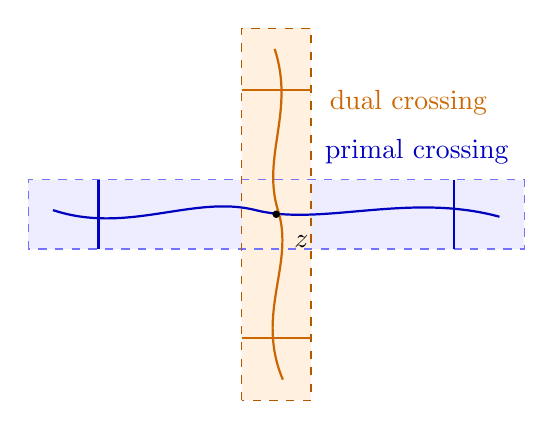
\begin{tikzpicture}[scale=1.05]
 \fill[blue!7] (-3,-.42) rectangle (3,.42);
 \fill[orange!12] (-.42,-2.25) rectangle (.42,2.25);
 \draw[blue!55,dashed] (-3,-.42) rectangle (3,.42);
 \draw[orange!70!black,dashed] (-.42,-2.25) rectangle (.42,2.25);
 \draw[blue!75!black,thick]
   (-2.7,.05) .. controls (-1.8,-.25) and (-1,.24) .. (-.25,.05)
   .. controls (.55,-.15) and (1.6,.27) .. (2.7,-.03);
 \draw[orange!80!black,thick]
   (.08,-2) .. controls (-.26,-1.2) and (.23,-.6) .. (.02,.05)
   .. controls (-.18,.7) and (.23,1.25) .. (-.02,2);
 \draw[blue!75!black,thick] (-2.15,-.42)--(-2.15,.42);
 \draw[blue!75!black,thick] (2.15,-.42)--(2.15,.42);
 \draw[orange!80!black,thick] (-.42,-1.5)--(.42,-1.5);
 \draw[orange!80!black,thick] (-.42,1.5)--(.42,1.5);
 \node[blue!75!black,anchor=south] at (1.7,.49) {primal crossing};
 \node[orange!80!black,anchor=west] at (.53,1.35) {dual crossing};
 \fill (0,0) circle (1.3pt);
 \node[anchor=north west] at (.1,-.14) {$z$};
\end{tikzpicture}
\caption{The two narrow tubes force transverse passages.  The drawing
shows only projected path ranges; it asserts neither injectivity of
the projection nor shape control of discrete edges.  The topological
input lifts this configuration to an intersection of a primal edge
with its paired dual edge.}
\label{nd:transverse-figure}
\end{figure}

\subsection{Uniformly bounded ring cutoffs}

We can now apply the annular construction in constant energy units,
rather than the hypothetical vanishing units used in the contradiction.

\begin{proposition}[Ring cutoffs]\label{nd:cutoffs}
Fix a compact subpatch of an ordinary chart and an aspect ratio
$\tau>1$.  Along a coupled further extraction from any rate sequence,
there is a constant $C$, depending only on the chart and $\tau$,
with the following property.  For every fixed disk
$\overline{B(z,\tau r)}$ contained with a margin in that subpatch,
both graphs eventually admit functions $\chi_m$ valued in $[0,1]$
such that
\[
 \chi_m=1\quad\text{on every lift of }\overline{B(z,r)},
 \qquad
 \chi_m=0\quad\text{on every lift outside }B(z,\tau r),
 \qquad
 \en(\chi_m)\le C
\]
on the primal graph, with $\enstar(\chi_m)\le C$ on the dual.
Their energy is supported in the indicated ring, up to vanishing
projected mesh.  The constant is independent of $z,r,m$; the
threshold in $m$ may depend on the fixed disk.  These assertions
hold simultaneously for the countable buffered disk tests, and
extend to arbitrary fixed disks by strict inner and outer margins.
\end{proposition}

\begin{proof}
Proposition~\ref{nd:nondegeneration} and the second quantile bound
in \eqref{nd:quantiles} give the barrier hypotheses with
deterministic units equal to one, at every fixed backward offset.
Choose an intermediate closed ring whose two radii lie strictly
between $r$ and $\tau r$, with all three resulting radial widths
comparable to $(\tau-1)r$.  Cover it by a finite union $U$ of open
boxes with closure strictly inside the target ring and area
$O_\tau(r^2)$.  Apply Lemma~\ref{nd:densities} to this $U$.
First choose $N$ so large that $R_N$ is small compared with the
intermediate width and both collars, and then take $m$ large.
The density is supported in the target ring.  Every full ring
crossing has a subcrossing through the intermediate ring,
confined to $U$, with advance comparable to $(\tau-1)r$.
The density therefore charges it by a fixed multiple of this
width.  After division by the width, the squared density norm
is bounded by $C(\tau)$ times the chart constant.
The clipped-distance construction of
Lemma~\ref{nd:el-traffic} gives the cutoff, with exact constants
on all inner and outer lifts.  One may carry out the construction
on a protected capped sphere and extend by constants beyond the
chart.  Only the ring density changes the function.

Countable buffered comparisons make all the fixed tests available
in one extraction.  A disk outside the chosen countable library
is handled by choosing a nearby library center, an inner library
disk containing $\overline{B(z,r)}$, and a concentric outer library
disk contained in $B(z,\tau r)$.  Their radii can be chosen
comparable to $r$, with constants depending only on $\tau$, and
their radial separation at least $c(\tau-1)r$.  The preceding
density estimate bounds the cutoff energy by a chart constant
times the squared ratio of outer radius to radial separation.
It therefore gives a uniform $C(\tau)$ for these library tests,
with the required constants on the original inner and outer
sets.  This use does not require a resolution threshold uniform
over all disk radii.
\end{proof}

All these conclusions are local in the actual conformal coordinate.
They therefore also hold in each fixed forward quantum-area offset
of Proposition~\ref{inp:transport}.  The joint cone zoom and
ordinary-patch exhaustion of \cite[Lemma ``From indexed Gaussian charts
to the whole cone'']{MetricMaps} let these patches exhaust the plane
away from its marked cone point.  Only probability-one conclusions
are transferred in this exhaustion.  The marked point will be
handled by removability when the variational limits are assembled.
